\documentclass[crop, tikz]{standalone}
\usepackage{tikz}
\usepackage{amsmath}
\usepackage{amssymb}

\usetikzlibrary{decorations.pathmorphing, positioning}

\definecolor{echodrk}{HTML}{0099cc}

\newcommand{\argmax}{\operatornamewithlimits{argmax}}

\begin{document}
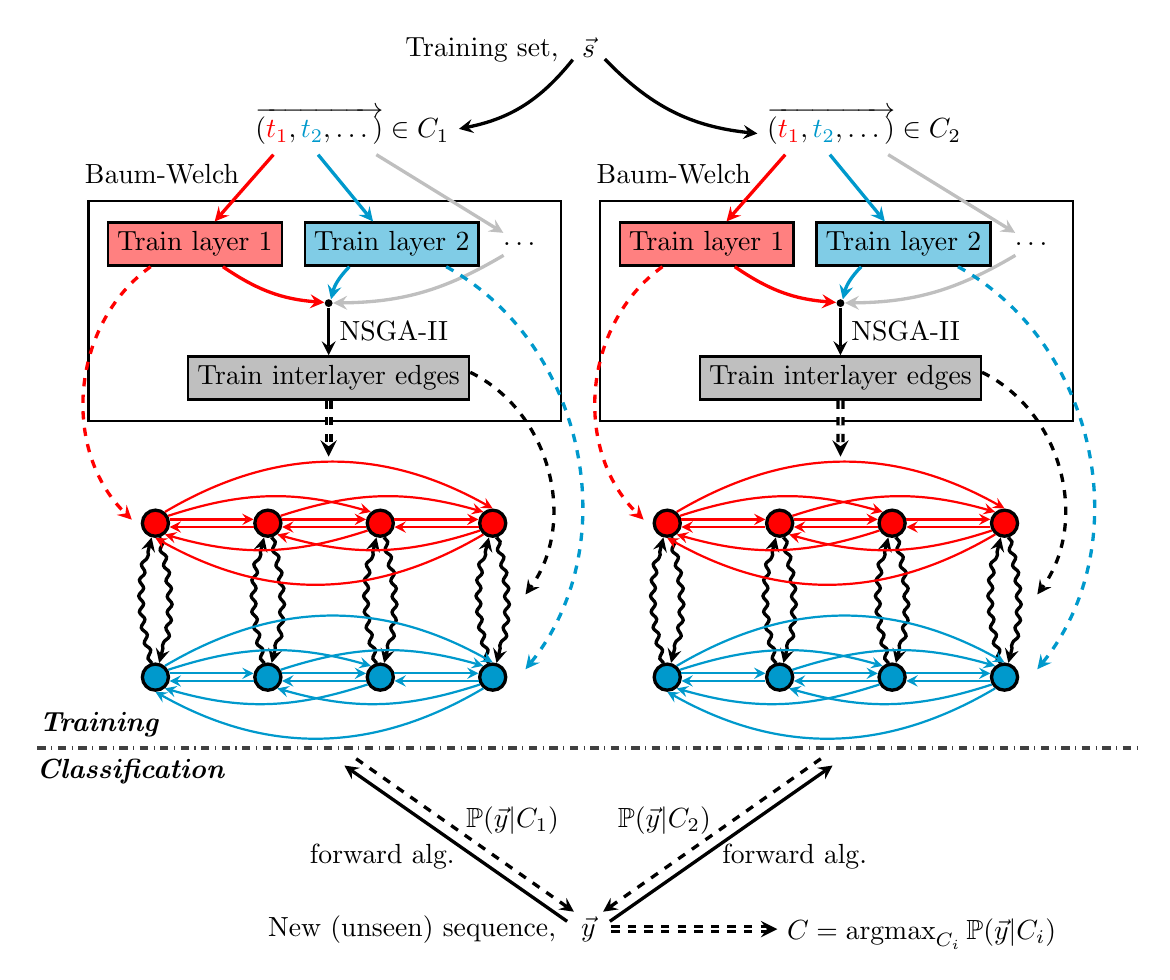
\begin{tikzpicture}[node distance=2.5cm]

	\draw[-, dashdotted, darkgray, very thick] (-2, -6.4) to (12, -6.4);
	\node[rectangle] at (-1.2, -6.1) {\emph{\textbf{Training}}};
	\node[rectangle] at (-0.8, -6.7) {\emph{\textbf{Classification}}};

	\node[circle, inner sep=0.2em, text depth=0em] (S) at (5, 2.5) {$\vec{s}$};
	\node[left = 0em of S, text depth=0em] (Slab) {Training set, };

	\node[rectangle] (out1) at (2,1.5) {$\overrightarrow{(\textcolor{red}{t_1}, \textcolor{echodrk}{t_2}, \dots)} \in C_1$};
	
	\node[rectangle] (out2) at (8.5,1.5) {$\overrightarrow{(\textcolor{red}{t_1}, \textcolor{echodrk}{t_2}, \dots)} \in C_2$};
	
	\draw[-stealth, very thick, bend left=20] (S) to (out1);
	\draw[-stealth, very thick, bend right=20] (S) to (out2);

	\node[rectangle, thick, draw, fill=red!50] (L1P) at (0, 0) {Train layer 1};
	\node[rectangle, thick, draw, fill=echodrk!50] (L2P) at (2.5, 0) {Train layer 2};
	\node[rectangle] (L3P) at (4.15, 0) {\dots};
	
	\node[circle,black,fill, inner sep=0.1em] (CP) at (1.7, -0.75){};
	
	\node[rectangle, thick, draw, fill=lightgray] (NP) at (1.7, -1.7) {Train interlayer edges};
	\node [draw,thick,minimum width=6cm,minimum height=2.8cm] (W1) at (1.65,-0.85) {};
	
	\begin{scope}[shift={(6.5,0)}]
		\node[rectangle, thick, draw, fill=red!50] (L1N) at (0, 0) {Train layer 1};
		\node[rectangle, thick, draw, fill=echodrk!50] (L2N) at (2.5, 0) {Train layer 2};
		\node[rectangle] (L3N) at (4.15, 0) {\dots};
		
		\node[circle,black,fill, inner sep=0.1em] (CN) at (1.7, -0.75){};
		
		\node[rectangle, thick, draw, fill=lightgray] (NN) at (1.7, -1.7) {Train interlayer edges};
		\node [draw,thick,minimum width=6cm,minimum height=2.8cm] (W2) at (1.65,-0.85) {};
	\end{scope}
	
	\draw[-stealth, very thick, red] (out1.200) to node[above left=-0.3em] {\textcolor{black}{Baum-Welch}} (L1P);
	\draw[-stealth, very thick, echodrk] (out1.220) to (L2P);
	\draw[-stealth, very thick, lightgray] (out1.310) to (L3P);
	
	\draw[-stealth, very thick, red, bend right=15] (L1P) to (CP);
	\draw[-stealth, very thick, echodrk, bend right=15] (L2P) to (CP);
	\draw[-stealth, very thick, lightgray, bend left=15] (L3P) to (CP);
	\draw[-stealth, very thick] (CP) to node[right] {NSGA-II} (NP);
	
	\draw[-stealth, dashed, red, very thick, bend right=50] (L1P) to (-0.8, -3.5);
	
	\draw[-stealth, dashed, echodrk, very thick, bend left=50] (L2P) to (4.2, -5.4);
	
	\draw[-stealth, dashed, very thick, bend left=50] (NP) to (4.2, -4.45);
	
	\draw[-stealth, double, dashed, very thick] (NP) to (1.7, -2.7);

	\draw[-stealth, very thick, red] (out2.200) to node[above left=-0.3em] {\textcolor{black}{Baum-Welch}} (L1N);
	\draw[-stealth, very thick, echodrk] (out2.220) to (L2N);
	\draw[-stealth, very thick, lightgray] (out2.310) to (L3N);
	
	\draw[-stealth, very thick, red, bend right=15] (L1N) to (CN);
	\draw[-stealth, very thick, echodrk, bend right=15] (L2N) to (CN);
	\draw[-stealth, very thick, lightgray, bend left=15] (L3N) to (CN);
	\draw[-stealth, very thick] (CN) to node[right] {NSGA-II} (NN);
	
	\draw[-stealth, dashed, red, very thick, bend right=50] (L1N) to (5.7, -3.5);
	
	\draw[-stealth, dashed, echodrk, very thick, bend left=50] (L2N) to (10.7, -5.4);
	
	\draw[-stealth, dashed, very thick, bend left=50] (NN) to (10.7, -4.45);
	
	\draw[-stealth, double, dashed, very thick] (NN) to (8.2, -2.7);
	
	\node[circle, draw, very thick, fill=echodrk] (111) at (-0.5, -5.5) {};
	\node[circle, draw, very thick, fill=echodrk, right=3em of 111] (222) {};
	\node[circle, draw, very thick, fill=echodrk, right=3em of 222] (333) {};
	\node[circle, draw, very thick, fill=echodrk, right=3em of 333] (444) {};
		
	\node[circle, draw, very thick, fill=red, above = 4.5em of 111] (1) {};
	\node[circle, draw, very thick, fill=red, right=3em of 1] (2) {};
	\node[circle, draw, very thick, fill=red, right=3em of 2] (3) {};
	\node[circle, draw, very thick, fill=red, right=3em of 3] (4) {};
		
	\draw[very thick, -stealth, decoration={snake, pre length=0.01mm, segment length=2mm, amplitude=0.3mm, post length=1.5mm}, decorate, bend left=15] (1) to (111);
	\draw[very thick, -stealth, decoration={snake, pre length=0.01mm, segment length=2mm, amplitude=0.3mm, post length=1.5mm}, decorate, bend left=15] (111) to (1);
		
	\draw[very thick, -stealth, decoration={snake, pre length=0.01mm, segment length=2mm, amplitude=0.3mm, post length=1.5mm}, decorate, bend left=15] (2) to (222);
	\draw[very thick, -stealth, decoration={snake, pre length=0.01mm, segment length=2mm, amplitude=0.3mm, post length=1.5mm}, decorate, bend left=15] (222) to (2);
		
	\draw[very thick, -stealth, decoration={snake, pre length=0.01mm, segment length=2mm, amplitude=0.3mm, post length=1.5mm}, decorate, bend left=15] (3) to (333);
	\draw[very thick, -stealth, decoration={snake, pre length=0.01mm, segment length=2mm, amplitude=0.3mm, post length=1.5mm}, decorate, bend left=15] (333) to (3);	
		
	\draw[very thick, -stealth, decoration={snake, pre length=0.01mm, segment length=2mm, amplitude=0.3mm, post length=1.5mm}, decorate, bend left=15] (4) to (444);
	\draw[very thick, -stealth, decoration={snake, pre length=0.01mm, segment length=2mm, amplitude=0.3mm, post length=1.5mm}, decorate, bend left=15] (444) to (4);
		
	\draw[-stealth, thick, bend left=17, color=echodrk] (111.30) to (333.130); % Consumption
	\draw[-stealth, thick, bend left=30, color=echodrk] (111.50) to (444.90); % Consumption
	\draw[-stealth, thick, bend left=17, color=echodrk] (222.30) to (444.130); % Consumption
		
	\draw[stealth-, thick, bend right=17, color=echodrk] (111.310) to (333.210); % Consumption
	\draw[stealth-, thick, bend right=30, color=echodrk] (111.270) to (444.230); % Consumption
	\draw[stealth-, thick, bend right=17, color=echodrk] (222.310) to (444.210); % Consumption
		
	\draw[stealth-, thick, color=echodrk] (111.345) to (222.195); % Consumption
	\draw[-stealth, thick, color=echodrk] (111.15) to (222.165); % Consumption
	\draw[stealth-, thick, color=echodrk] (222.345) to (333.195); % Consumption
	\draw[-stealth, thick, color=echodrk] (222.15) to (333.165); % Consumption
	\draw[stealth-, thick, color=echodrk] (333.345) to (444.195); % Consumption
	\draw[-stealth, thick, color=echodrk] (333.15) to (444.165); % Consumption
		
	\draw[-stealth, thick, bend left=17, color=red] (1.30) to (3.130); % Consumption
	\draw[-stealth, thick, bend left=30, color=red] (1.50) to (4.90); % Consumption
	\draw[-stealth, thick, bend left=17, color=red] (2.30) to (4.130); % Consumption
		
	\draw[stealth-, thick, bend right=17, color=red] (1.310) to (3.210); % Consumption
	\draw[stealth-, thick, bend right=30, color=red] (1.270) to (4.230); % Consumption
	\draw[stealth-, thick, bend right=17, color=red] (2.310) to (4.210); % Consumption
		
	\draw[stealth-, thick, color=red] (1.345) to (2.195); % Consumption
	\draw[-stealth, thick, color=red] (1.15) to (2.165); % Consumption
	\draw[stealth-, thick, color=red] (2.345) to (3.195); % Consumption
	\draw[-stealth, thick, color=red] (2.15) to (3.165); % Consumption
	\draw[stealth-, thick, color=red] (3.345) to (4.195); % Consumption
	\draw[-stealth, thick, color=red] (3.15) to (4.165); % Consumption
  
	\begin{scope}[shift={(6.5,0)}]
		\node[circle, draw, very thick, fill=echodrk] (N111) at (-0.5, -5.5) {};
		\node[circle, draw, very thick, fill=echodrk, right=3em of N111] (N222) {};
		\node[circle, draw, very thick, fill=echodrk, right=3em of N222] (N333) {};
		\node[circle, draw, very thick, fill=echodrk, right=3em of N333] (N444) {};
		
		\node[circle, draw, very thick, fill=red, above = 4.5em of N111] (N1) {};
		\node[circle, draw, very thick, fill=red, right=3em of N1] (N2) {};
		\node[circle, draw, very thick, fill=red, right=3em of N2] (N3) {};
		\node[circle, draw, very thick, fill=red, right=3em of N3] (N4) {};
		
		\draw[very thick, -stealth, decoration={snake, pre length=0.01mm, segment length=2mm, amplitude=0.3mm, post length=1.5mm}, decorate, bend left=15] (N1) to (N111);
		\draw[very thick, -stealth, decoration={snake, pre length=0.01mm, segment length=2mm, amplitude=0.3mm, post length=1.5mm}, decorate, bend left=15] (N111) to (N1);
		
		\draw[very thick, -stealth, decoration={snake, pre length=0.01mm, segment length=2mm, amplitude=0.3mm, post length=1.5mm}, decorate, bend left=15] (N2) to (N222);
		\draw[very thick, -stealth, decoration={snake, pre length=0.01mm, segment length=2mm, amplitude=0.3mm, post length=1.5mm}, decorate, bend left=15] (N222) to (N2);
		
		\draw[very thick, -stealth, decoration={snake, pre length=0.01mm, segment length=2mm, amplitude=0.3mm, post length=1.5mm}, decorate, bend left=15] (N3) to (N333);
		\draw[very thick, -stealth, decoration={snake, pre length=0.01mm, segment length=2mm, amplitude=0.3mm, post length=1.5mm}, decorate, bend left=15] (N333) to (N3);
		
		\draw[very thick, -stealth, decoration={snake, pre length=0.01mm, segment length=2mm, amplitude=0.3mm, post length=1.5mm}, decorate, bend left=15] (N4) to (N444);
		\draw[very thick, -stealth, decoration={snake, pre length=0.01mm, segment length=2mm, amplitude=0.3mm, post length=1.5mm}, decorate, bend left=15] (N444) to (N4);
		
		\draw[-stealth, thick, bend left=17, color=echodrk] (N111.30) to (N333.130);
		\draw[-stealth, thick, bend left=30, color=echodrk] (N111.50) to (N444.90);
		\draw[-stealth, thick, bend left=17, color=echodrk] (N222.30) to (N444.130);
		
		\draw[stealth-, thick, bend right=17, color=echodrk] (N111.310) to (N333.210);
		\draw[stealth-, thick, bend right=30, color=echodrk] (N111.270) to (N444.230);
		\draw[stealth-, thick, bend right=17, color=echodrk] (N222.310) to (N444.210);
		
		\draw[stealth-, thick, color=echodrk] (N111.345) to (N222.195);
		\draw[-stealth, thick, color=echodrk] (N111.15) to (N222.165); 
		\draw[stealth-, thick, color=echodrk] (N222.345) to (N333.195); 
		\draw[-stealth, thick, color=echodrk] (N222.15) to (N333.165); 
		\draw[stealth-, thick, color=echodrk] (N333.345) to (N444.195); 
		\draw[-stealth, thick, color=echodrk] (N333.15) to (N444.165); 
				
		\draw[-stealth, thick, bend left=17, color=red] (N1.30) to (N3.130);
		\draw[-stealth, thick, bend left=30, color=red] (N1.50) to (N4.90);
		\draw[-stealth, thick, bend left=17, color=red] (N2.30) to (N4.130);
		
		\draw[stealth-, thick, bend right=17, color=red] (N1.310) to (N3.210);
		\draw[stealth-, thick, bend right=30, color=red] (N1.270) to (N4.230);
		\draw[stealth-, thick, bend right=17, color=red] (N2.310) to (N4.210);
		
		\draw[stealth-, thick, color=red] (N1.345) to (N2.195);
		\draw[-stealth, thick, color=red] (N1.15) to (N2.165);
		\draw[stealth-, thick, color=red] (N2.345) to (N3.195);
		\draw[-stealth, thick, color=red] (N2.15) to (N3.165);
		\draw[stealth-, thick, color=red] (N3.345) to (N4.195);
		\draw[-stealth, thick, color=red] (N3.15) to (N4.165);	
	\end{scope}
  
	\node[circle, inner sep=0.2em] (Y) at (5, -8.7) {$\vec{y}$};
	\node[left = 0em of Y] (Ylab) {New (unseen) sequence, };
	
	\node[circle] (imag1) at (1.9, -6.45) {};
	\node[circle] (imag2) at (8.1, -6.45) {};
	
	\draw[-stealth, very thick] (Y.160) to node[below left=-0.5em] {forward alg.} (imag1.270);
	\draw[-stealth, very thick] (Y.20) to node[below right=-0.5em] {forward alg.} (imag2.270);
	
	\draw[stealth-, dashed, very thick] (Y.130) to node[above right=-0.5em] {$\mathbb{P}(\vec{y}|C_1)$} (imag1.330);
	\draw[stealth-, dashed, very thick] (Y.50) to node[above left=-0.5em] {$\mathbb{P}(\vec{y}|C_2)$} (imag2.210);
  
	\node[rectangle, right= 6em of Y, text depth=0em] (ret) {$C = \argmax_{C_i} \mathbb{P}(\vec{y}|C_i)$};
	\draw[-stealth, double, dashed, very thick] (Y) to (ret);
\end{tikzpicture}
\end{document}
